\begin{table}[t]
\caption{EnHi-LMP dataset statistics}\label{tab:data}
\centering\footnotesize
\begin{tabular}{@{}lrrr@{}}
\toprule
 & Insurance & Tenancy & Total\\
\midrule
English pairs & 80 & 80 & 160\\
Hindi pairs & 80 & 80 & 160\\
Faithful / single-error & 80 / 80 & 80 / 80 & 160 / 160\\
Preserved / Partial / Not (gold) & -- & -- & 160 / 20 / 140\\
Sanity: identical / unrelated & -- & -- & 160 / 160\\
\midrule
\multicolumn{4}{@{}l}{\footnotesize Error types (EN+HI): scope 22, omitted condition 20, date 20,}\\
\multicolumn{4}{@{}l}{\footnotesize modality 16, minor 16, hallucination 16, party 16, negation 14,}\\
\multicolumn{4}{@{}l}{\footnotesize exception 12, number 8.}\\
\bottomrule
\end{tabular}
\end{table}

\section{Experimental Setup}
\textbf{Protocol.} E1 uses 5-fold cross-validation \emph{grouped by clause}: the English and Hindi twins of a clause, and both of its simplifications, always fall in the same fold, so no test clause is seen in training in either language. Learned models are run with three seeds; we report the mean and standard deviation of each metric computed over the pooled out-of-fold predictions. E2 splits the clauses into two halves and trains on one language of one half while testing on the other language of the other half (and the in-language controls). E3 trains on one domain and tests on the other, and additionally evaluates on the official FrJUDGE test split (90 French pairs with \emph{human} LMP labels, mean of five annotators), either zero-shot from EnHi-LMP or after training on FrJUDGE train+dev (207 pairs). E4 scores the 320 held-out sanity pairs with the E1 models, including a hybrid model trained without augmentation. E5 applies the explainer to the out-of-fold scores of the best model.

\textbf{Metrics.} Pearson $r$, Spearman $\rho$, RMSE and MAE against the gold LMP; macro-F1 of the three-way decision; F1 of the ``Not preserved'' class; and precision, recall and F1 of the error-type classifier.

\section{Results}
\subsection{E1: Generic similarity vs.\ LMP models}
Table~\ref{tab:e1} shows that the best generic metric is chrF ($r=0.37$); embedding cosine and token alignment reach only $0.18$. Because these similarities vary little between faithful and corrupted rewrites, their calibrated predictions cluster in the middle of the scale and almost never cross the ``Not preserved'' threshold (NP-F1 $\le 0.25$). LegalDiff-GBR is the best system on every metric ($r=0.60$, RMSE $2.94$, NP-F1 $0.61$). The JUDGEBERT-style cross-encoder trained from scratch does not learn a useful signal from 256 training pairs on its own ($r=0.12$); fusing LegalDiff raises it to $0.44$. H1 is therefore supported for legal-aware modelling, but not yet for the encoder alone.

\begin{table}[t]
\caption{E1: 5-fold grouped CV on EnHi-LMP ($n=320$)}\label{tab:e1}
\centering\footnotesize\setlength{\tabcolsep}{3pt}
\resizebox{\columnwidth}{!}{%
\begin{tabular}{@{}lcccccc@{}}
\toprule
System & $r\uparrow$ & $\rho\uparrow$ & RMSE$\downarrow$ & MAE$\downarrow$ & Dec.F1$\uparrow$ & NP-F1$\uparrow$\\
\midrule
chrF & 0.37 & 0.36 & 3.38 & 3.00 & 0.28 & 0.25 \\
Embedding cosine & 0.18 & 0.16 & 3.58 & 3.38 & 0.06 & 0.06 \\
Token-align.\ F1 & 0.18 & 0.19 & 3.58 & 3.39 & 0.04 & 0.00 \\
\midrule
LegalDiff-GBR & \textbf{0.60\,{\scriptsize$\pm$0.01}} & \textbf{0.58} & \textbf{2.94} & \textbf{2.24} & \textbf{0.53} & \textbf{0.61} \\
ML-JudgeBERT (text) & 0.12\,{\scriptsize$\pm$0.01} & 0.08 & 4.50 & 3.45 & 0.35 & 0.37 \\
ML-JudgeBERT+LegalDiff & 0.44\,{\scriptsize$\pm$0.02} & 0.45 & 3.82 & 2.63 & 0.42 & 0.46 \\
\bottomrule
\end{tabular}}
\end{table}

\subsection{E2: English vs.\ Hindi}
Table~\ref{tab:lang} breaks E1 down by language and domain. The generic embedding metrics lose almost half of their correlation on Hindi (cosine $0.38\rightarrow0.21$; token alignment $0.42\rightarrow0.28$): the English-centric tokenizer splits Devanagari into characters, so unrelated Hindi sentences look similar. LegalDiff-GBR is language-stable ($0.60$ vs.\ $0.59$). In cross-lingual transfer (Table~\ref{tab:transfer}) LegalDiff-GBR trained on English reaches $r=0.48$ on Hindi and, trained on Hindi, $0.54$ on English, close to the in-language controls ($0.50$ and $0.55$), whereas embedding cosine collapses to $0.04$ on Hindi.

\begin{table}[t]
\caption{Pearson $r$ by language and domain (E1/E2)}\label{tab:lang}
\centering\footnotesize
\begin{tabular}{@{}lcccc@{}}
\toprule
System & EN & HI & Insurance & Tenancy\\
\midrule
chrF & 0.36 & 0.38 & 0.36 & 0.38 \\
Embedding cosine & 0.38 & 0.21 & 0.17 & 0.19 \\
Token-align.\ F1 & 0.42 & 0.28 & 0.13 & 0.22 \\
\midrule
LegalDiff-GBR & 0.60 & 0.59 & 0.59 & 0.61 \\
ML-JudgeBERT (text) & 0.10 & 0.13 & 0.10 & 0.13 \\
ML-JudgeBERT+LegalDiff & 0.41 & 0.46 & 0.36 & 0.51 \\
\bottomrule
\end{tabular}
\end{table}

\begin{table*}[t]
\caption{E2/E3: Transfer across language, domain and to human-labelled FrJUDGE (Pearson $r$)}\label{tab:transfer}
\centering\footnotesize
\begin{tabular}{@{}lcccccc@{}}
\toprule
Train $\rightarrow$ test & chrF & Emb.\ cosine & Token-align.\ F1 & LegalDiff-GBR & ML-JudgeBERT (text) & ML-JudgeBERT+LegalDiff\\
\midrule
EN$\rightarrow$HI & 0.39 & 0.04 & 0.16 & \textbf{0.48} & 0.08 & 0.36 \\
HI$\rightarrow$EN & 0.37 & 0.26 & 0.24 & \textbf{0.54} & 0.06 & 0.42 \\
EN$\rightarrow$EN & 0.37 & 0.35 & 0.42 & \textbf{0.55} & 0.11 & 0.39 \\
HI$\rightarrow$HI & 0.37 & 0.25 & 0.28 & \textbf{0.50} & 0.14 & 0.34 \\
\midrule
Ins.$\rightarrow$Ten. & 0.40 & 0.20 & 0.22 & \textbf{0.55} & 0.19 & 0.51 \\
Ten.$\rightarrow$Ins. & 0.36 & 0.17 & 0.14 & \textbf{0.57} & 0.26 & 0.38 \\
\midrule
EnHi$\rightarrow$FrJUDGE & 0.47 & -0.17 & 0.03 & 0.56 & 0.23 & \textbf{0.59} \\
FrJUDGE$\rightarrow$FrJUDGE & 0.47 & -0.17 & 0.03 & \textbf{0.60} & 0.22 & 0.48 \\
\bottomrule
\end{tabular}
\end{table*}

\subsection{E3: New domain and out-of-language transfer}
Training on insurance and testing on tenancy, or the reverse, costs LegalDiff-GBR at most $0.06$ in $r$ relative to in-domain cross-validation (Tables~\ref{tab:lang}--\ref{tab:transfer}). The most informative result is on FrJUDGE, whose labels are genuine human judgements: models trained \emph{only} on EnHi-LMP reach $r=0.56$ (LegalDiff-GBR) and $0.59$ (ML-JudgeBERT+LegalDiff), above chrF ($0.47$), while embedding cosine is negatively correlated ($-0.17$). Trained on FrJUDGE itself, LegalDiff-GBR reaches $r=0.60$ with RMSE $1.96$. Note that LegalDiff includes a small French lexicon (Section~\ref{sec:limits}).

\subsection{E4: Sanity checks}
Table~\ref{tab:sanity} reports mean predictions on identical (gold 10) and unrelated (gold 1) pairs. Models trained with augmentation give identical pairs $\approx10$ and unrelated pairs $1.2$--$1.7$; chrF behaves correctly on identical pairs but rates unrelated pairs $2.9$. Embedding similarity fails both checks after calibration and gives unrelated \emph{Hindi} pairs $6.6/10$. The text-only encoder places unrelated pairs at $4.8$. Removing augmentation from the hybrid model changes little because LegalDiff already separates these extremes.

\begin{table}[t]
\caption{E4: Sanity checks (mean $\hat{y}$; share within tolerance)}\label{tab:sanity}
\centering\footnotesize\setlength{\tabcolsep}{3pt}
\resizebox{\columnwidth}{!}{%
\begin{tabular}{@{}lcccc@{}}
\toprule
System & Ident. & $\ge9$ & Unrel. & $\le2$\\
\midrule
chrF & 10.00 & 100\% & 2.89 & 4\% \\
Embedding cosine & 7.10 & 0\% & 4.36 & 20\% \\
Token-align.\ F1 & 7.15 & 0\% & 5.20 & 0\% \\
LegalDiff-GBR & 9.99 & 100\% & 1.22 & 94\% \\
ML-JudgeBERT (text) & 9.41 & 80\% & 4.78 & 19\% \\
ML-JudgeBERT+LegalDiff & 9.98 & 100\% & 1.70 & 82\% \\
ML-JudgeBERT+LegalDiff, no aug. & 9.92 & 99\% & 1.88 & 74\% \\
\bottomrule
\end{tabular}}
\end{table}

\subsection{E5: Error analysis and explanations}
Fig.~\ref{fig:err} shows mean predictions per gold error type. Embedding cosine assigns roughly 6--7 to every type, i.e.\ it cannot separate a faithful rewrite from a negation, a changed number or a swapped party. LegalDiff-GBR tracks the gold profile, with the clearest separation for negation, numbers, dates, exceptions and omitted conditions, and the weakest for scope changes and hallucinated content, which have no dedicated lexical marker.

Using the out-of-fold LegalDiff-GBR scores, the explainer detects that a legal error is present with precision $0.74$, recall $0.85$ and F1 $0.79$. It names the exact error type for $40\%$ of all corrupted pairs ($47\%$ of those it flags), with an 11-class macro-F1 of $0.41$ (Table~\ref{tab:explain}). Exceptions ($0.67$), dates ($0.58$), parties ($0.51$), numbers ($0.50$) and modality ($0.49$) are explained best; scope changes are never typed correctly.

Table~\ref{tab:cases} lists 18 legally difficult cases: the 16 error pairs that embedding similarity over-scores most (at most one per type and language) and two faithful paraphrases with low lexical overlap. Typical successes are polarity reversals expressed with \hi{नहीं} in Hindi (case 3) and figure or deadline changes (cases 12--13). Typical failures are (i) polarity changed through the verb rather than a negator (``does not cover'' $\rightarrow$ ``pays for'', case 7), (ii) party swaps that keep the same role words (case 6) and (iii) a faithful Hindi paraphrase that reorders the clause and is wrongly flagged (case 17).

\begin{figure}[t]
\centering
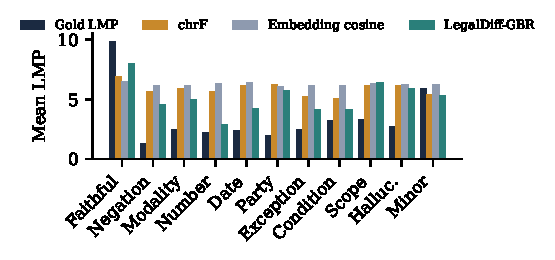
\includegraphics[width=\columnwidth]{fig_errtype.pdf}
\caption{E5: mean LMP by gold error type (out-of-fold predictions, EN+HI).}\label{fig:err}
\end{figure}

\begin{table}[t]
\caption{E5: Error-type explanation quality (LegalDiff-GBR scores)}\label{tab:explain}
\centering\footnotesize
\begin{tabular}{@{}lcccc@{}}
\toprule
Type & $n$ & P & R & F1\\
\midrule
\textsc{none} & 160 & 0.82 & 0.69 & 0.75 \\
\textsc{scope} & 22 & 0.00 & 0.00 & 0.00 \\
\textsc{date} & 20 & 0.61 & 0.55 & 0.58 \\
\textsc{omit\_cond} & 20 & 0.32 & 0.30 & 0.31 \\
\textsc{entity} & 16 & 0.37 & 0.81 & 0.51 \\
\textsc{halluc} & 16 & 0.18 & 0.12 & 0.15 \\
\textsc{minor} & 16 & 0.23 & 0.44 & 0.30 \\
\textsc{modality} & 16 & 0.43 & 0.56 & 0.49 \\
\textsc{negation} & 14 & 0.20 & 0.50 & 0.29 \\
\textsc{exc\_removed} & 12 & 1.00 & 0.50 & 0.67 \\
\textsc{number} & 8 & 0.75 & 0.38 & 0.50 \\
\bottomrule
\end{tabular}
\end{table}

\begin{table*}[t]
\caption{E5: Qualitative analysis of 18 legally difficult cases (scores on the 1--10 LMP scale; $^{\times}$ = wrong predicted type)}\label{tab:cases}
\centering\footnotesize\setlength{\tabcolsep}{4pt}
\begin{tabular}{@{}rllp{7.4cm}rrrrrl@{}}
\toprule
\# & Lang & Gold type & Legal change (original $\rightarrow$ simplification) & Gold & chrF & Emb. & GBR & Hybrid & Predicted type\\
\midrule
1 & HI & \textsc{modality} & ``must not'' use for hire unless covered $\rightarrow$ ``may'' use unless excluded & 1 & 6.2 & 7.1 & 4.2 & 9.2 & \textsc{scope}$^{\times}$ \\
2 & HI & \textsc{entity} & benefit goes to nominee on policyholder's death $\rightarrow$ roles swapped & 1 & 7.6 & 7.0 & 5.2 & 6.2 & \textsc{entity} \\
3 & HI & \textsc{negation} & landlord shall not cut water/power $\rightarrow$ may cut if rent unpaid & 1 & 7.2 & 7.0 & 4.5 & 9.3 & \textsc{negation} \\
4 & HI & \textsc{omit\_cond} & entry after 24-h notice, 8 a.m.--8 p.m. $\rightarrow$ any time, no notice & 1 & 4.2 & 6.9 & 2.7 & 1.3 & \textsc{negation}$^{\times}$ \\
5 & HI & \textsc{halluc} & eviction only by legal procedure $\rightarrow$ after 7 days' notice & 1 & 5.0 & 6.8 & 6.0 & 1.4 & \textsc{entity}$^{\times}$ \\
6 & EN & \textsc{entity} & benefit goes to nominee on policyholder's death $\rightarrow$ roles swapped & 1 & 8.3 & 6.5 & 7.9 & 9.9 & \textsc{none}$^{\times}$ \\
7 & EN & \textsc{negation} & ``does not cover'' wear and tear $\rightarrow$ ``pays for'' it & 1 & 8.8 & 6.1 & 8.9 & 9.9 & \textsc{none}$^{\times}$ \\
8 & HI & \textsc{date} & newborn covered from 91st day $\rightarrow$ from day of birth & 2 & 5.6 & 7.1 & 5.1 & 8.1 & \textsc{date} \\
9 & HI & \textsc{exc\_removed} & liable for damage, wear and tear excepted $\rightarrow$ including wear and tear & 2 & 5.7 & 7.0 & 5.4 & 5.3 & \textsc{exc\_removed} \\
10 & HI & \textsc{scope} & insurer pays rateable share $\rightarrow$ pays entire loss & 2 & 5.4 & 7.0 & 5.9 & 9.1 & \textsc{minor}$^{\times}$ \\
11 & HI & \textsc{number} & deposit $\le$ 2 months' rent $\rightarrow$ $\le$ 6 months' rent & 2 & 4.9 & 6.9 & 2.3 & 1.1 & \textsc{date}$^{\times}$ \\
12 & EN & \textsc{date} & six-month lock-in $\rightarrow$ three-month lock-in & 2 & 7.2 & 6.6 & 5.5 & 10.0 & \textsc{date} \\
13 & EN & \textsc{number} & deductible Rs 5,000 $\rightarrow$ Rs 50,000 & 2 & 8.4 & 6.6 & 5.3 & 9.4 & \textsc{number} \\
14 & EN & \textsc{omit\_cond} & entry after 24-h notice, 8 a.m.--8 p.m. $\rightarrow$ any time, no notice & 1 & 4.6 & 5.4 & 3.5 & 1.1 & \textsc{date}$^{\times}$ \\
15 & EN & \textsc{halluc} & eviction only by legal procedure $\rightarrow$ after 7 days' notice & 1 & 5.0 & 5.4 & 3.6 & 1.0 & \textsc{modality}$^{\times}$ \\
16 & EN & \textsc{exc\_removed} & no hazardous goods except cooking gas $\rightarrow$ including cooking gas & 2 & 7.7 & 6.1 & 7.6 & 9.8 & \textsc{none}$^{\times}$ \\
17 & HI & \textsc{none} & faithful: rent +5\% after every 11 months & 10 & 2.0 & 6.2 & 1.8 & 5.4 & \textsc{halluc}$^{\times}$ \\
18 & EN & \textsc{none} & faithful: rent +5\% after every 11 months & 10 & 3.2 & 5.2 & 9.0 & 7.1 & \textsc{none} \\
\bottomrule
\end{tabular}
\end{table*}

\section{Discussion}
\textbf{Does the model capture legal meaning better than generic similarity?} Yes, when legal differences are modelled explicitly. LegalDiff-GBR beats every generic metric in every setting we tested: overall, per language, across domains and on French human judgements, and on decision F1 and sanity checks. The hybrid model beats them overall and on FrJUDGE, but not in every slice (e.g.\ English: $0.41$ vs.\ $0.42$ for token alignment; HI$\rightarrow$HI: $0.34$ vs.\ $0.37$ for chrF). Generic similarity is especially unreliable for Hindi, where English-centric subword vocabularies degrade to characters.

\textbf{Why does the encoder underperform?} JUDGEBERT fine-tunes an encoder that already knows the language; our encoder had to learn English, Hindi and legal semantics from 256 pairs. Its weak standalone result is evidence for pretraining, not against cross-encoding: once given LegalDiff it becomes competitive and is the best system on zero-shot FrJUDGE.

\section{Limitations}\label{sec:limits}
(1) Gold scores are rubric-based silver labels written by the authors; inter-annotator agreement has not yet been measured, so absolute numbers may be optimistic, especially because LegalDiff's categories mirror the error taxonomy. The FrJUDGE results, based on independent human labels, partly address this. (2) Each corrupted pair contains one controlled error; naturally produced simplifications may combine several. (3) The encoder was trained from scratch for lack of pretrained checkpoints. (4) LegalDiff's lexicons are hand-built for English and Hindi, with a small French list (74 entries) added only for the FrJUDGE check. (5) Evaluation is sentence-level without document context.

\section{Conclusion and Future Work}
We extended JUDGEBERT's legal meaning preservation task to English and Hindi and to tenancy law, released a 320-pair parallel dataset with typed legal errors and sanity sets, and showed that generic similarity is not a legal-meaning metric ($r\le0.37$). Explicit, bilingual legal-difference modelling gives the strongest and most transferable signal ($r=0.60$ in-domain; $0.56$ zero-shot on human-labelled French data) and produces typed explanations (error-detection F1 $0.79$). Next steps are double human annotation with Krippendorff's $\alpha$, fine-tuning XLM-R and MuRIL backbones on GPU, LLM-generated simplifications with multiple errors, and paragraph-level context.

\section*{Acknowledgment}
We thank Dr.\ Surabhi Solanki for guidance, and the JUDGEBERT authors for releasing FrJUDGE and their code.
